\begin{frame}{Y86-64: convenience for hardware}
\begin{columns}[t]
\begin{column}{0.5\textwidth}
\vspace{0cm}
\begin{itemize}
    \item 4 bits to decode instruction size/layout
    \item (mostly) uniform placement of operands
    \item jumping to zeroes (uninitialized?) by accident halts
    \item no attempt to fit (parts of) multiple instructions in a byte
\end{itemize}
\end{column}
\begin{column}{0.5\textwidth}
\vspace{0cm}
\begin{adjustbox}{max size={\textwidth}{\textheight}}
\begin{tikzpicture}
\tikzset{extra box shorter width/.style={text width=.025cm}}
\instrEncodingTable
\end{tikzpicture}
\end{adjustbox}
\vspace{0cm}
\end{column}
\end{columns}
\end{frame}

\usetikzlibrary{calc}

\begin{frame}{on uniform placement}
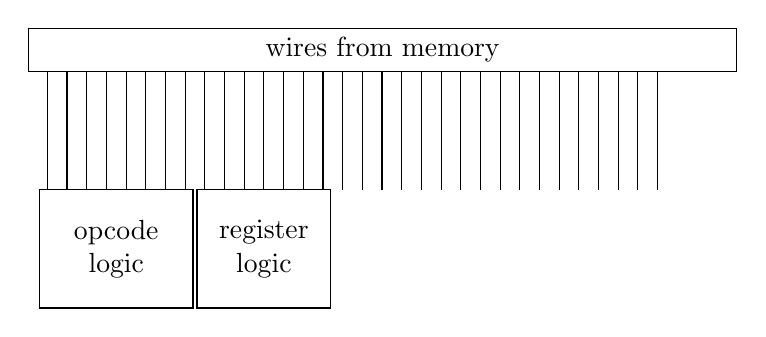
\begin{tikzpicture}
\node[draw,minimum width=9cm] (instr) {wires from memory};
\foreach \x in {1,2,3,4,...,32} {
    \draw ($(instr.south west) + (.25*\x, 0)$) -- ++(0, -1.5) coordinate (bottom \x);
}
\draw ([xshift=-.1cm]bottom 1) rectangle ([xshift=.1cm,yshift=-1.5cm]bottom 8) node[align=center,midway] { opcode \\ logic };
\draw ([xshift=-.1cm]bottom 9) rectangle ([xshift=.1cm,yshift=-1.5cm]bottom 15) node[align=center,midway] { register \\ logic };
\end{tikzpicture}
\begin{adjustbox}{max size={0.3\textwidth}{0.3\textheight}}
\begin{tikzpicture}
\instrEncodingTable
\end{tikzpicture}
\end{adjustbox}
\begin{itemize}
\item simpler hardware: directly wire memory bits to where needed
\item disadvantage: ``wasted'' space in instructions 
    \begin{itemize}
    \item e.g. 0s and Fs in Y86
    \item and more space with fixed-length instruction sets
    \end{itemize}
\end{itemize}
\end{frame}

\begin{frame}{on variable size}
\begin{adjustbox}{max size={0.5\textwidth}{0.5\textheight}}
\begin{tikzpicture}
\instrEncodingTable
\end{tikzpicture}
\end{adjustbox}
    \begin{itemize}
    \item future: want to run instructions in parallel
    \item problem with Y86: need to read one instruction to even find next
        \begin{itemize}
        \item but at least only need to process 4 bits
        \end{itemize}
    \end{itemize}
\end{frame}
